\documentclass{beamer}
\usepackage[utf8]{inputenc}
\usepackage[T1]{fontenc}
\usepackage{graphicx}
\usepackage{tcolorbox}
\usepackage{hyperref}
\hypersetup{
    colorlinks=true,
    linkcolor=pink,
    urlcolor=cyan,
    urlbordercolor=cyan,
}
\graphicspath{ {./images/} }

\usetheme{Arguelles}

\title{Tutorial 9}
\subtitle{CS3241 Computer Graphics (AY22/23)}
\date{\today}
\author{Wong Pei Xian}
\institute[]{\email{e0389023@u.nus.edu}}

\begin{document}

\frame[plain]{\titlepage}


\section{Question 1}

\begin{frame}
    \frametitle{Question 1}
    Considering the rendering efficiency and rendering quality on a standard polygon-based rasterization 
    renderer, what are the disadvantages of representing surfaces using polygon mesh compared to using 
    Bézier patches?
\end{frame}

\begin{frame}
    \frametitle{Adaptive subdivision}

    De Casteljau's algorithm can be used to \textbf{generate polygons} adaptively.\\
    Less screen space $\Rightarrow$ less levels of subdivision $\Rightarrow$ less vertices.\\
    More screen space $\Rightarrow$ more levels of subdivision $\Rightarrow$ more vertices.\\

    \vspace{1em}

    \begin{center}
        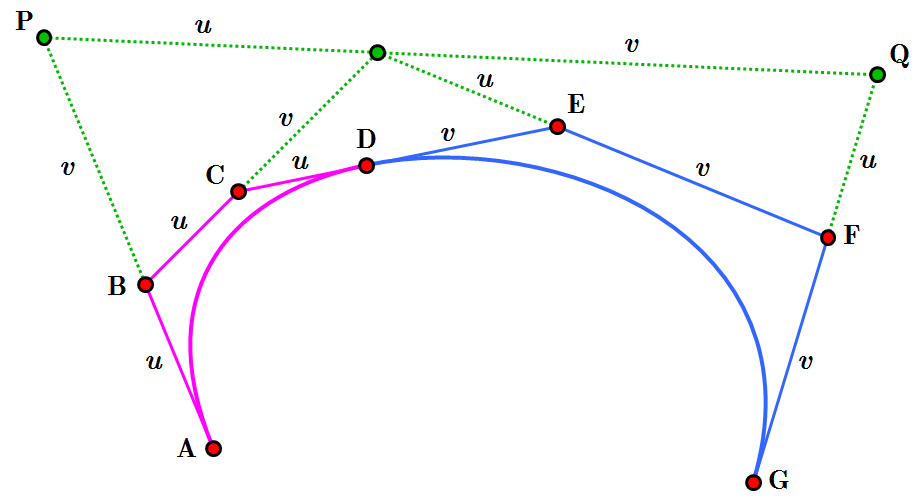
\includegraphics[scale=0.4]{q1-adaptive-subdiv.png}
    \end{center}

\end{frame}

\begin{frame}
    \frametitle{Adaptive subdivision}

    Compared to polygon mesh which has \textbf{fixed vertex/polygon count}, facing:
    \begin{itemize}
        \item poorer efficiency for small meshes which need less vertices
        \item poorer fidelity for large meshes which cannot achieve smooth curves 
    \end{itemize}

\end{frame}

\section{Question 2}

\begin{frame}
    \frametitle{Question 2}
    Propose a way to measure the “flatness” of a cubic Bézier curve segment in 2D space. 
    Can your method be extended to a cubic Bézier curve segment in 3D space?
\end{frame}

\begin{frame}
    \frametitle{Convex hull}

    \begin{center}
        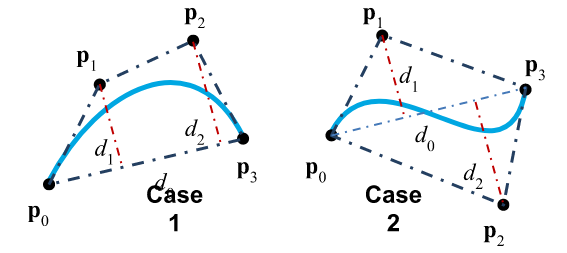
\includegraphics[]{q2-types-of-curves.png}
    \end{center}

\end{frame}

\begin{frame}
    \frametitle{Flatness estimate $f$}

    \begin{center}
        \textbf{Case 1}: $f = \max(d_1, d_2)$\\
        \textbf{Case 2}: $f = \max(d_1, d_2)$
    \end{center}

    \begin{tcolorbox}
        Q: How to determine cases 1 or 2?\\
        A: determine if the intersection of the lines formed by $p_1 p_2$ and 
        $p_0 p_3$ lies within $p_0, p_3$
    \end{tcolorbox}

\end{frame}

\section{Question 3}

\begin{frame}
    \frametitle{Question 3}
    Propose a way to measure the “flatness” of a cubic Bézier \textbf{surface patch}.
\end{frame}

\begin{frame}
    \frametitle{Extending Q2}

    \begin{center}
        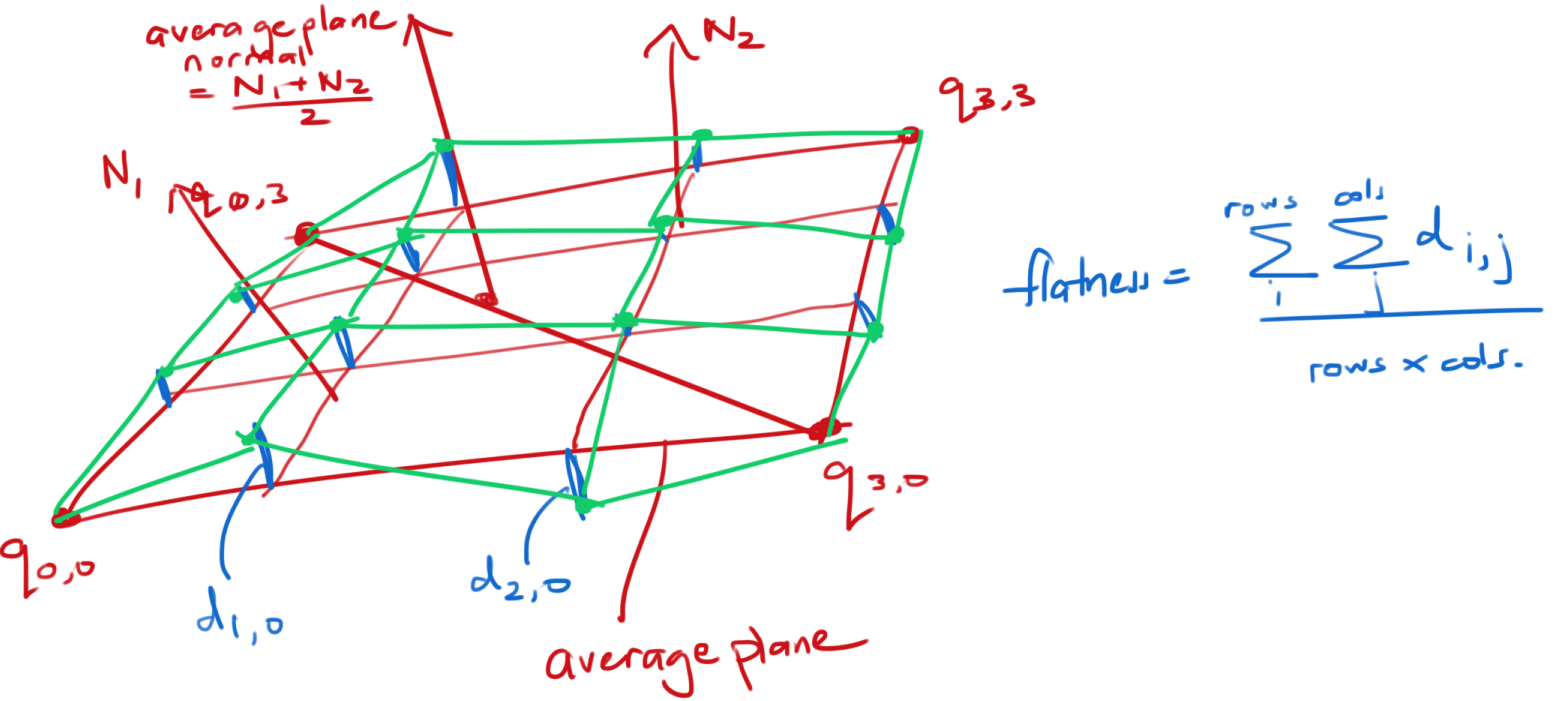
\includegraphics[scale=0.3]{q3.png}
    \end{center}

    Define the "average plane" (in red) as $N \cdot p = N \cdot \frac{q_{0,0} + q_{0,3} + q_{3,0} + q{3,3}}{4}$.
    \textit{(where $N$ is the average of the two normals of $q_{0,0}, q_{0,3}, q_{3,0}$ and $q_{3,0}, q_{0,3}, q_{3,3}$)}.
    
    \vspace{1em}
    \begin{tcolorbox}
        "Flatness" = average of distance between average plane and each point.
    \end{tcolorbox}

\end{frame}

\iffalse
\section{Recap: Parametric}

\begin{frame}[plain, standout]
    \AlegreyaExtraBold \LARGE
    Parametric Curves and Surfaces:\\
    Polynomial and Bezier
\end{frame}

\begin{frame}
    \frametitle{Parametric Curves/Surfaces}

    \begin{tcolorbox}
        Curve (2D):
        \begin{center}
            In \textbf{2D} space: $p(u) = \left[\begin{matrix} x(u) \\ y(u) \end{matrix}\right]$; \hspace{0.3em}
            In \textbf{3D} space: $p(u) = \left[\begin{matrix} x(u) \\ y(u) \\ z(u) \end{matrix}\right]$\\
        \end{center}
        where $x(u), y(u)$ can be any function of \textbf{single parameter} $u$.
    \end{tcolorbox}

    \vspace{0.5em}

    \begin{tcolorbox}
        Surface (3D):
        \begin{center}
            $p(u) = \left[\begin{matrix} x(u,v) \\ y(u,v) \\ z(u,v) \end{matrix}\right]$\\
        \end{center}
        where $x(u,v), y(u,v), z(u,v)$ can be any function of \textbf{two parameters}$ u, v$.
    \end{tcolorbox}
\end{frame}

\begin{frame}
    \frametitle{Parameteric Cubic Polynomial Curves}

    \begin{eqnarray*}
        p(u) =& c_0 + c_1 (u) + c_2 (u^2) + c_3 (u^3) \\
             =& 
            \begin{bmatrix}
                1 & u & u^2 & u^3
            \end{bmatrix}
            \begin{bmatrix}
                c_{0,x} & c_{0,y} & c_{0,z} \\
                c_{1,x} & c_{1,y} & c_{1,z} \\
                c_{2,x} & c_{2,y} & c_{2,z} \\
                c_{3,x} & c_{3,y} & c_{3,z}
            \end{bmatrix}\\
            =& 
            \begin{bmatrix}
                x(u) & y(u) & z(u)
            \end{bmatrix}
    \end{eqnarray*}

\end{frame}

\begin{frame}
    \frametitle{Cubic interpolating}

    Pre-determine points that \textbf{curve passes through} at $u = 0, \frac{1}{3}, \frac{2}{3}, 1$.

    \begin{center}
        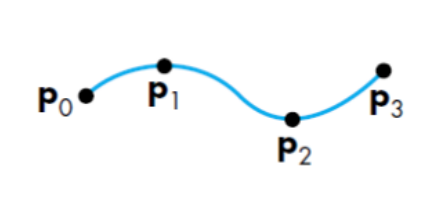
\includegraphics[scale=0.7]{cubic-interpolating.png}
    \end{center}

    Our conditions are for $k \in \{0 \dots 3\}$

    \begin{eqnarray*}
        p_k =& p(\frac{k}{3})\\
        =& c_0 + \frac{k}{3}c_1 + \left(\frac{k}{3}\right)^2c_2 + \left(\frac{k}{3}\right)^3 c_3
    \end{eqnarray*}

\end{frame}

\begin{frame}
    \centering
    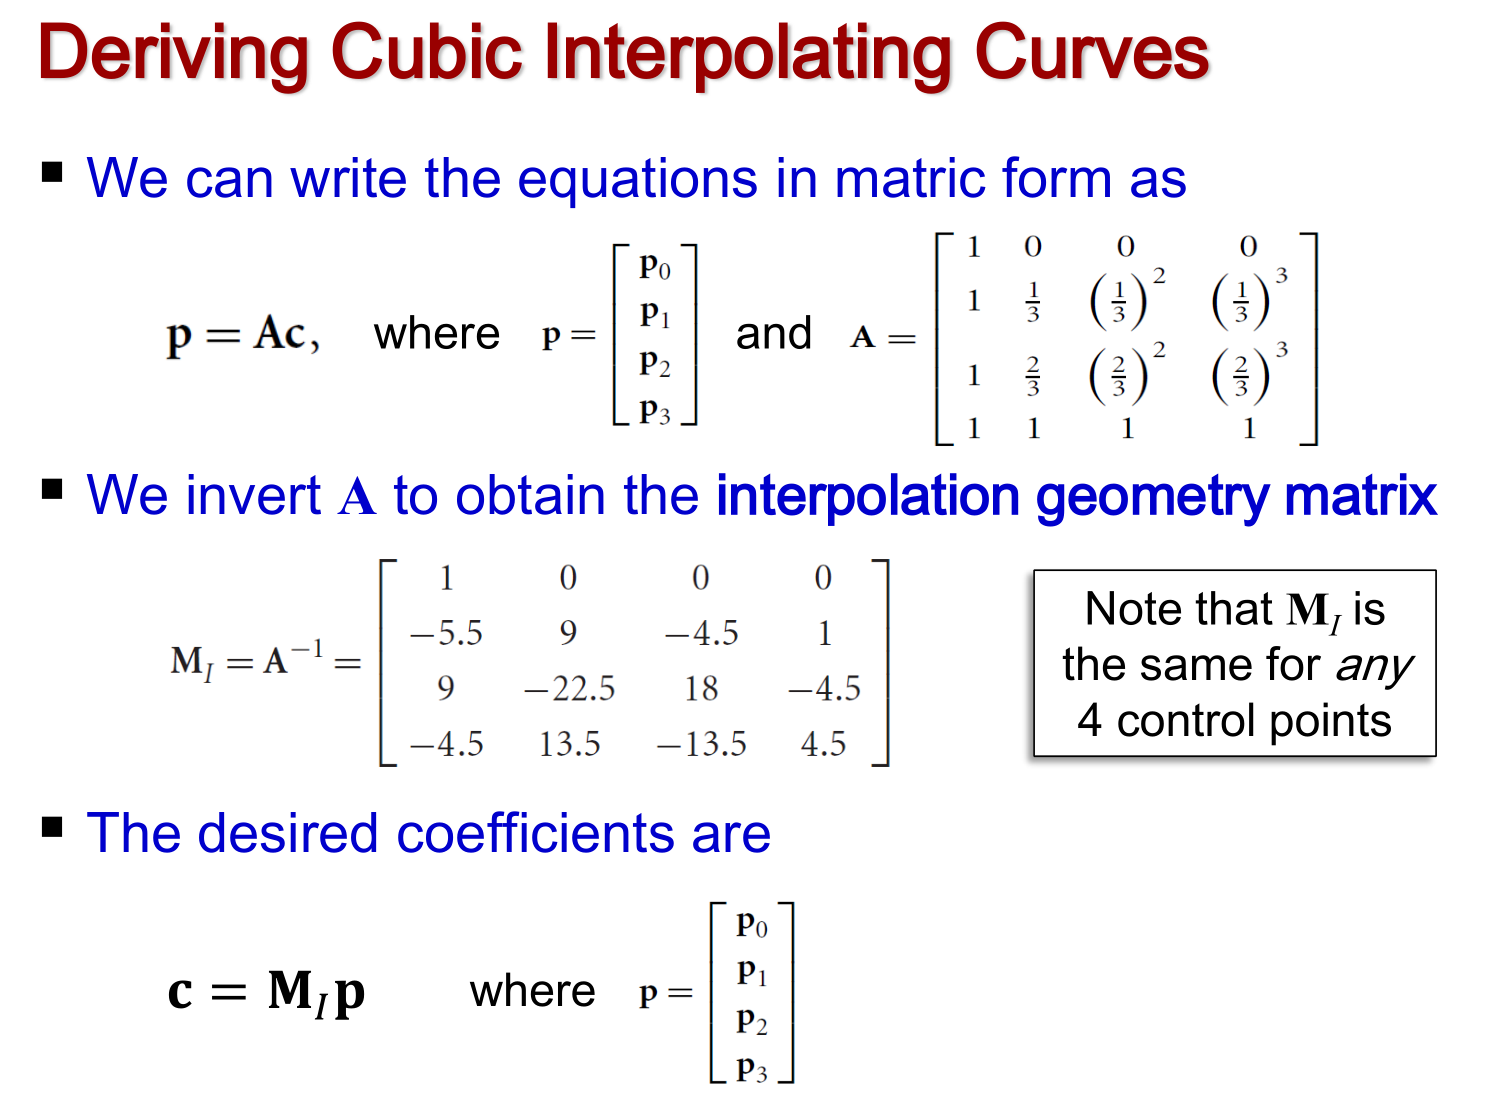
\includegraphics[scale=0.4]{derive-cubic-interpolating.png}
\end{frame}

\begin{frame}
    \frametitle{Cubic Bézier curves}
    
    Pre-determine points that \textbf{define the graph where}

    \begin{eqnarray*}
        p(0) =& p_0\\
        p(1) =& p_3\\
        p'(0) =& 3(p_1 - p_0)\\
        p'(1) =& 3(p_3 - p_2)
    \end{eqnarray*}

    Our conditions are

    \begin{eqnarray}
        p_0 =& c_0\\
        3p_1 - 3p_0 =& c_1\\
        3p_3 - 3p_2 =& c_1 + c_2 + c_3\\
        p_1 =& c_0 + c_1 + c_2 + c_3\\
    \end{eqnarray}

    \textit{Can you derive (1) and (2)?}
\end{frame}

\begin{frame}[plain, standout]
    \AlegreyaExtraBold \LARGE
    Blending functions and geometry matrices
\end{frame}

\begin{frame}
    \frametitle{Relationships between $p$ and $c$}

    \begin{equation*}
        \begin{bmatrix}
            p_0 \\ p_1 \\ p_2 \\ p_3
        \end{bmatrix} = A \begin{bmatrix}
            c_0 \\ c_1 \\ c_2 \\ c_3
        \end{bmatrix}
    \end{equation*}
    Here $A$ contains our conditions for the curve type (Bezier/interpolating).\\
    \vspace{1em}
    \textcolor{red}{However we usually define our points $p$ instead of $c$, and we want to derive $c$ instead.}
    We can do so by

    \begin{equation*}
        c_k = A^{-1}C = M_I p_k \text{ for interpolating, or }  M_B p_k \text{ for Bezier}
    \end{equation*}

\end{frame}

\begin{frame}
    \frametitle{Blending functions}

    \begin{eqnarray*}
        p(u) =& 
            \begin{bmatrix}
                1 & u & u^2 & u^3
            \end{bmatrix}
            \begin{bmatrix}
                c_{0} \\ c_{1} \\ c_{2} \\ c_{3}
            \end{bmatrix}\\
            =&
            \begin{bmatrix}
                1 & u & u^2 & u^3
            \end{bmatrix} M_I \begin{bmatrix}
                p_0 \\ p_1 \\ p_2 \\ p_3
            \end{bmatrix}\\
            =&
            \begin{bmatrix}
                b_0 & b_1 & b_2 & b_3
            \end{bmatrix}
            \begin{bmatrix}
                p_0 \\ p_1 \\ p_2 \\ p_3
            \end{bmatrix}\\
    \end{eqnarray*}

    \textcolor{red}{Our $b(u) = \begin{bmatrix}
        b_0(u) & b_1(u) & b_2(u) & b_3(u)
    \end{bmatrix}^T$}.

\end{frame}
\fi

\section{Question 4}

\begin{frame}
    \frametitle{Question 4}
    Given 4 control points $p_0, p_1, p_2, p_3$ for a cubic Bézier curve segment $p(u)$, 
    find the 4 control points $q_0, q_1, q_2, q_3$ for the cubic interpolating curve segment $q(u)$
    such that $q(u) = p(u)$.
\end{frame}

\begin{frame}
    \frametitle{Cubic Bézier to Cubic interpolating}

    The corresponding $q_k = q(\frac{k}{3}) = p(\frac{k}{3})$ \textit{(since $q(u) = p(u)$)}.
     
    \begin{eqnarray*}
        q(0) =& p_0\\
        q(\frac{1}{3}) =& p(\frac{1}{3})\\
        q(\frac{2}{3}) =& p(\frac{2}{3})\\
        q(1) =& p_1\\
    \end{eqnarray*}

    Directly compute $q$ from $p$.

\end{frame}

\section{Question 5}

\begin{frame}
    \frametitle{Question 5}
    Given 4 control points $q_0, q_1, q_2, q_3$ for the cubic interpolating curve segment $q(u)$,
    find the 4 control points $p_0, p_1, p_2, p_3$ for a cubic Bézier curve segment $p(u)$
    such that $p(u) = q(u)$.
\end{frame}

\begin{frame}
    \frametitle{Cubic interpolating to Cubic bezier}

    Let's look at our constraints:

    \begin{eqnarray*}
        p(0) =& p_0\\
        p(1) =& p_3\\
        p'(0) =& 3(p_1 - p_0)\\
        p'(1) =& 3(p_3 - p_2)
    \end{eqnarray*}

\end{frame}

\begin{frame}
    \frametitle{Cubic interpolating to Cubic bezier}

    Now we use the fact that $p(u) = q(u)$:

    \begin{eqnarray*}
        p_0 = p(0) =& \textcolor{red}{q(0) = q_0}\\
        p_3 = p(1) =& \textcolor{red}{q(1) = q_3}\\
        p'(0) =& \textcolor{red}{q'(0)} = 3(p_1 - p_0)\\
        p'(1) =& \textcolor{red}{q'(1)} = 3(p_3 - p_2)\\
    \end{eqnarray*}

    For $p_1, p_2$ we obtain them via:
    \begin{equation*}
        q'(0) = 3(p_1 - p_0) \Rightarrow \frac{q'(0)}{3} + p_0 = p_1
    \end{equation*}
    and
    \begin{equation*}
        q'(1) = 3(p_3 - p_2) \Rightarrow p_3 - \frac{q'(1)}{3} = p_2
    \end{equation*}
\end{frame}

\section{Question 6}

\begin{frame}
    \frametitle{Question 6}
    Given two cubic Bezier curve segments, $p(u)$ and $q(u)$, that are to be joined together, where $p(1) = q(0)$. 
    The control points of $p(u)$ are $p_0, p_1, p_2, p_3$ and the control points of $q(u)$ are $q_0, q_1, q_2, q_3$. 
    How should the control points of $q(u)$ be positioned so that there is $C^1$ continuity at the join point of $p(u)$ and $q(u)$?
\end{frame}

\begin{frame}
    \frametitle{Continuity}

    \centering
    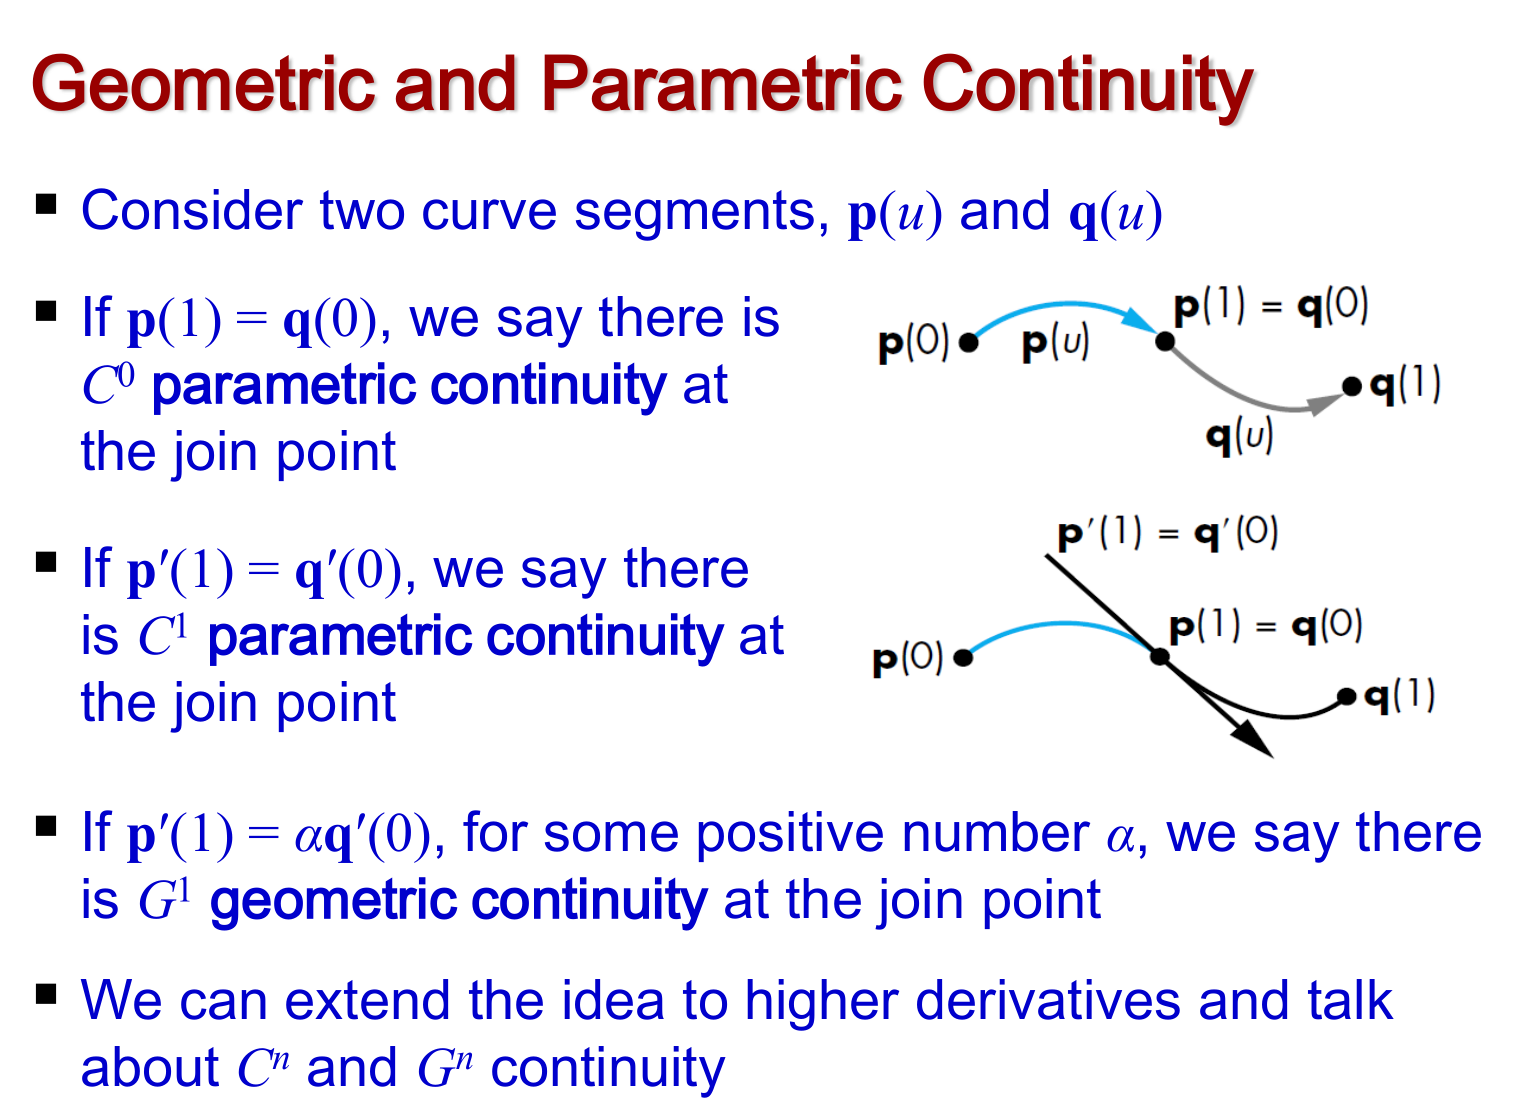
\includegraphics[scale=0.3]{continuity.png}

\end{frame}

\begin{frame}
    \frametitle{$C^1$ continuity}

    \begin{enumerate}
        \item $p(1) = p(0)$
        \item First derivative of $p$ at end = first derivative of $q$ at start: $p'(1) = q'(0)$.
    \end{enumerate}
    
    \begin{tcolorbox}
        \begin{eqnarray*}
            p(1) &=& \textcolor{teal}{p_3 = q_0} = q(0) \\
            p'(1) &=& \textcolor{teal}{3(p_3 - p_2) = 3(q_1 - q_0)} = q'(0)
        \end{eqnarray*}
    \end{tcolorbox}

\end{frame}

\section{Question 7}
\begin{frame}
    \frametitle{Question 7}
    Sketch two 2D curves that have $C^0$ continuity but not $C^1$ continuity.
\end{frame}

\begin{frame}
    \frametitle{Question 8}

    \centering
    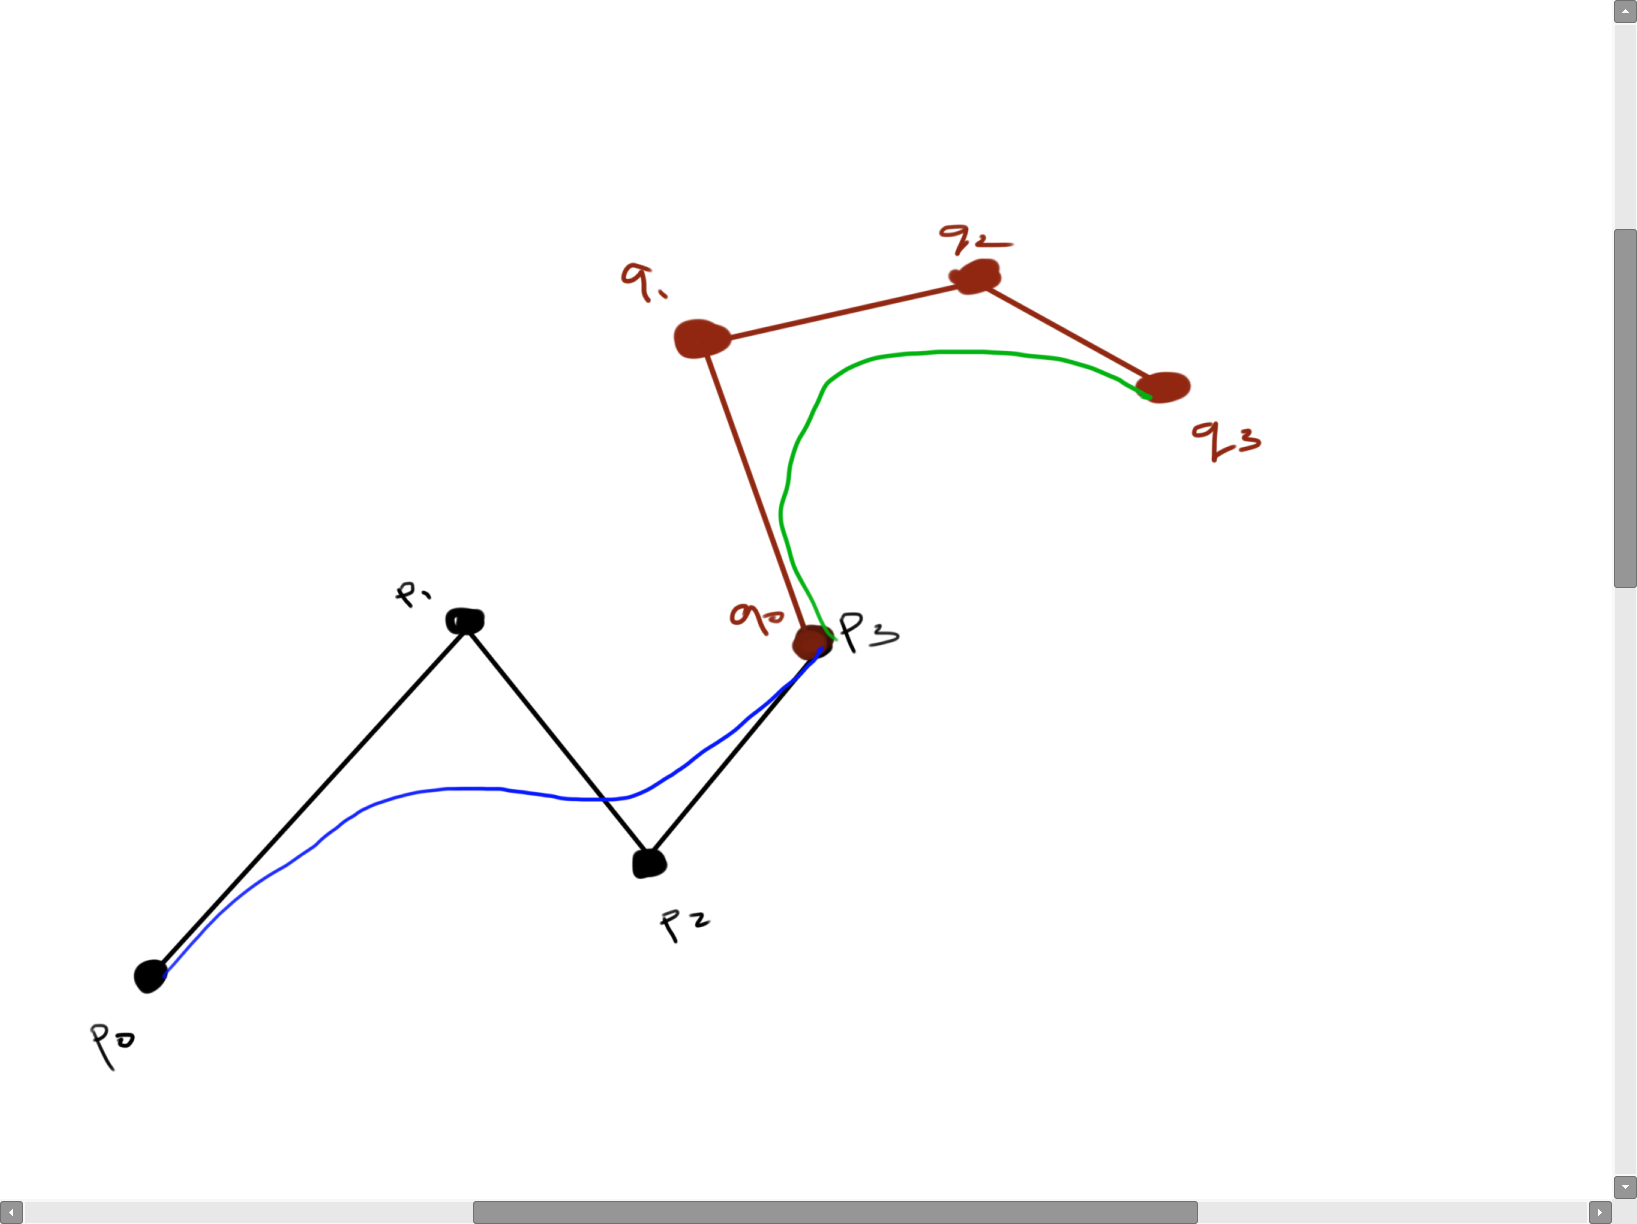
\includegraphics[scale=0.2]{q7.png}
    \vspace{1em}

    $C^0$ as both curves are joined $p_3 = q_0$.\\
    Not $C^1$ as $p'(1) \neq q'(0)$.

\end{frame}

\section{Question 8}

\begin{frame}
    \frametitle{Question 8}
    Sketch two 2D curves that have $C^1$ continuity but not $C^0$ continuity. Is it even possible to have such a situation?
\end{frame}

\begin{frame}
    \frametitle{Question 8}

    \centering
    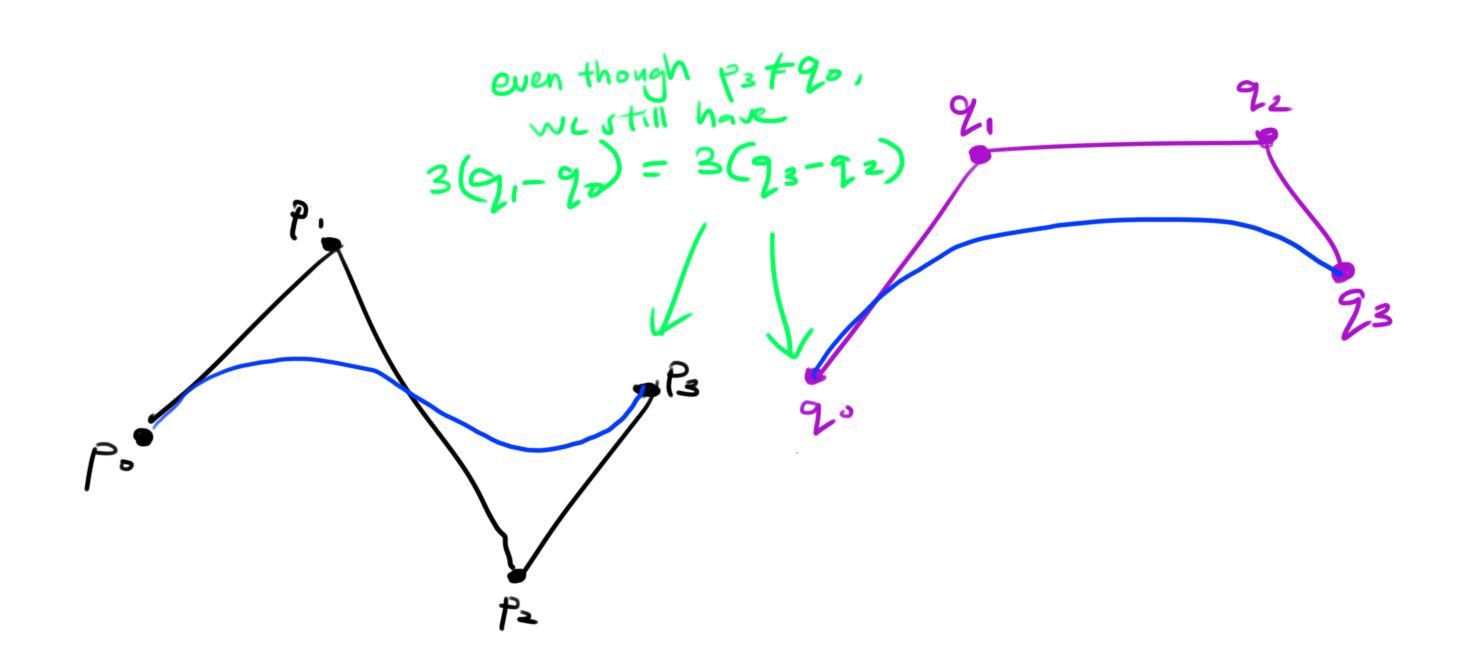
\includegraphics[scale=0.4]{q8.png}
    \vspace{1em}

    $C^1$ as $p'(1) = q'(0)$.\\
    Not $C^0$ as $p(1) \neq q(0)$.

\end{frame}

\section{Question 9}

\begin{frame}
    \frametitle{Question 9}
    Given 4 control points $p_0, p_1, p_2, p_3$ for a cubic Bézier curve segment $p(u)$, and any $0 \le u \le 1$
    show that the De Casteljau algorithm produces the point $p(u)$.

    \begin{tcolorbox}
        \begin{equation}
            p(u) = (1–u^)3 p_0 + 3u (1–u)^2 p_1 + 3u^2 (1–u) p_2 + u^3 p_3
        \end{equation}
    \end{tcolorbox}
\end{frame}

\begin{frame}
    \frametitle{De Casteljau's Algorithm}

    \begin{center}
        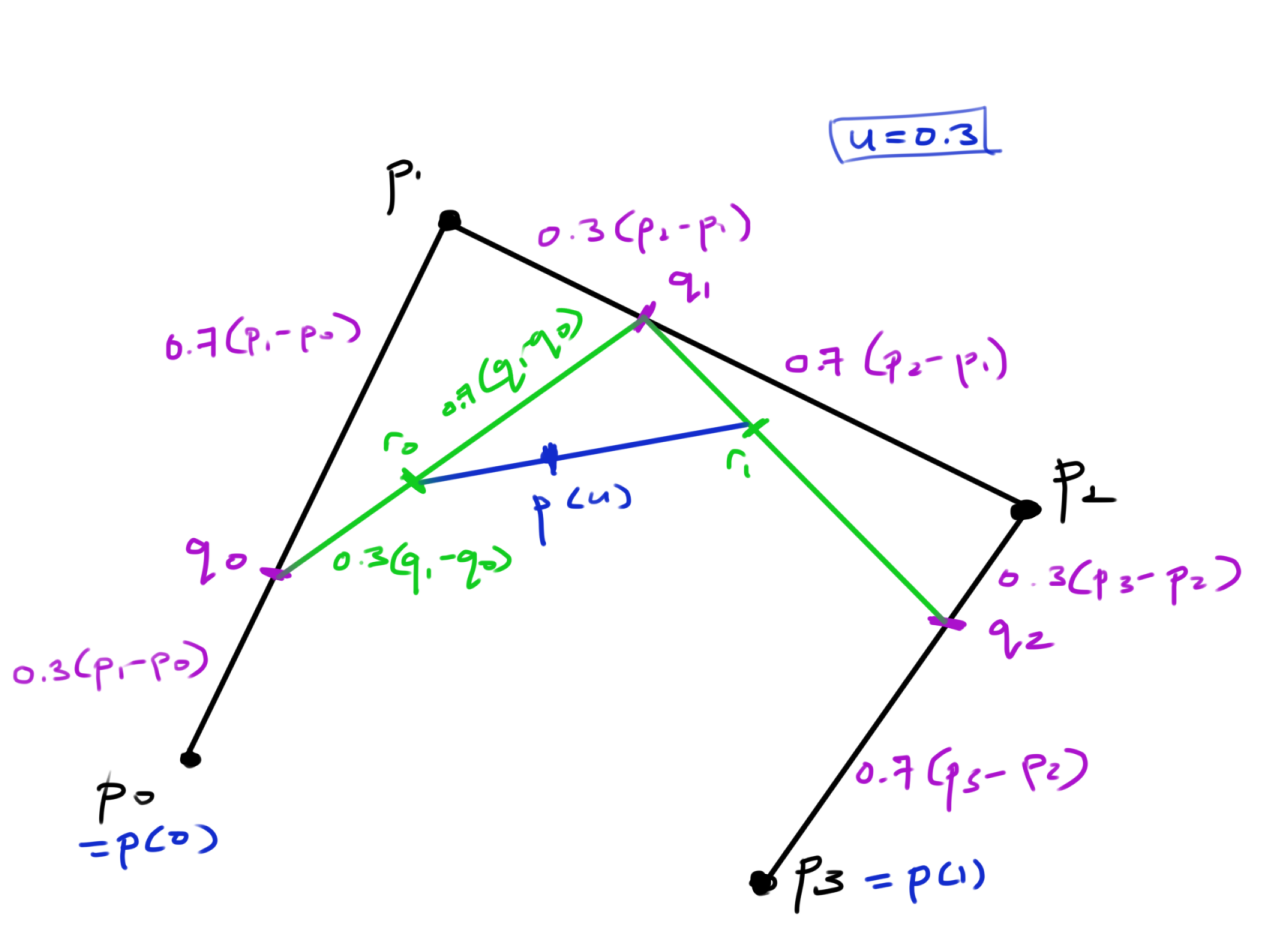
\includegraphics[scale=0.4]{q9-decasteljau.png}
    \end{center}

\end{frame}

\begin{frame}
    \frametitle{Approach: Unpack the Lerps}

    \begin{tcolorbox}
        Linear Interpolation of degree $t$ along points $a, b$:
        \begin{equation}
            \mathrm{lerp}(t, a, b) = (1 - t)a + b
        \end{equation}
    \end{tcolorbox}

\end{frame}

\begin{frame}
    \frametitle{Unpacked all lerps}

    \begin{center}
        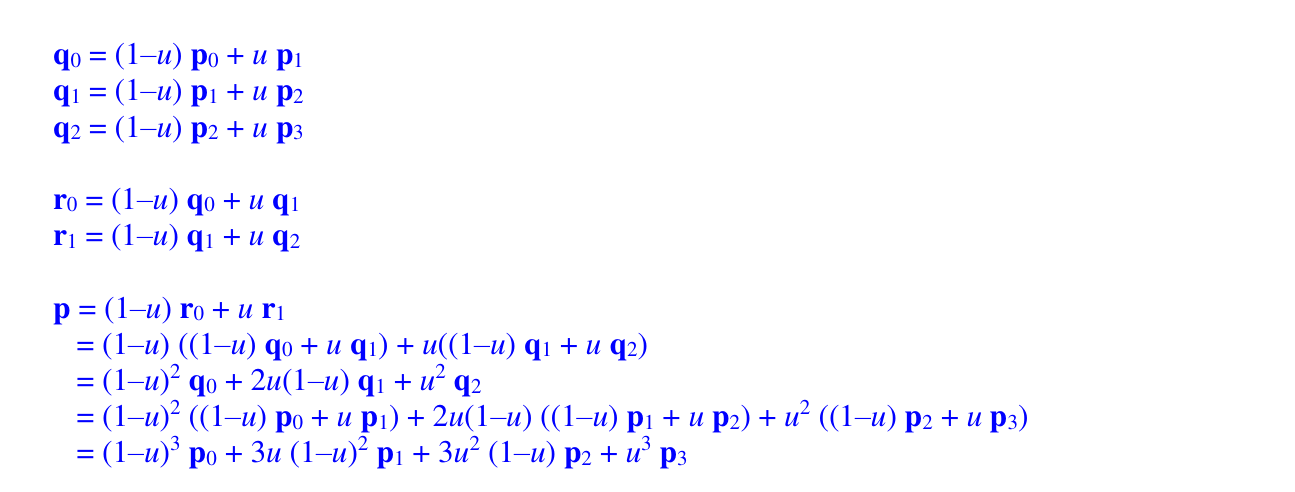
\includegraphics[width=\linewidth]{derive-bezier.png}
    \end{center}

\end{frame}

\begin{frame}
    \frametitle{Pseudocode}

    \begin{center}
        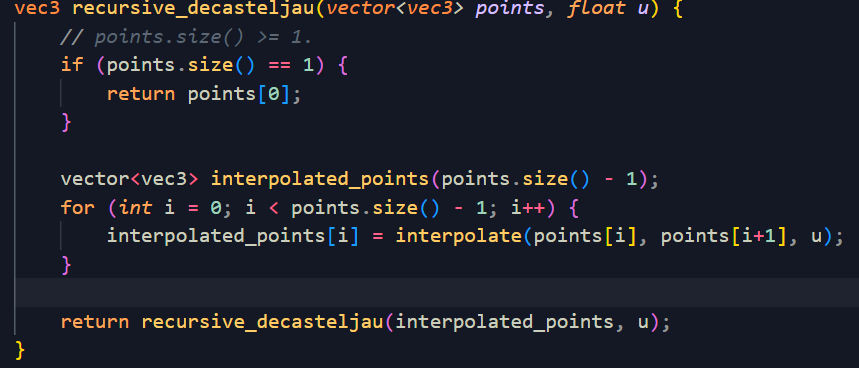
\includegraphics[scale=0.7]{q9-pseudocode.png}
    \end{center}

\end{frame}

\begin{frame}[plain,standout]
    \AlegreyaExtraBold \LARGE
    Attendance taking
\end{frame}

\ThankYou
\begin{frame}[plain,standout]
    Thanks! Get the slides here after the tutorial.\\
    \vspace{2em}
    \scalebox{3}{\faGithub}\par\bigskip
    \url{https://trxe.github.io/cs3241-notes}
\end{frame}

\end{document}